\documentclass{beamer}

\usepackage{microtype}
\usepackage{hyperref}
\usepackage[english]{babel}
\usepackage[utf8]{inputenc}
\usepackage[T1]{fontenc}
\usepackage{tikz}
% \usepackage{verbatim}
% \usepackage{fancyvrb}
\usepackage{listings}
\usepackage{courier}
\usepackage{tikz}
\usepackage{graphicx}

% \usefonttheme{serif} % default family is serif
% \usepackage{fontspec}
% \setmainfont{Liberation Serif}

\usetikzlibrary{positioning, fit, matrix, decorations.pathreplacing, shadows}
\lstset{basicstyle=\ttfamily\footnotesize,breaklines=true}

\mode<presentation>
{
  % \usetheme{Marburg}
  % \usetheme{Montpellier}
  % \usetheme{Hannover}
  % \usetheme{Berkeley}
  \usetheme{Antibes}
  % or ...

  % \setbeamercovered{transparent}
  % or whatever (possibly just delete it)
}

% todo: real mode vs protected mode.
\title{Build \& boot the Linux kernel}
\author{Chandan \& Vasant}
\date{}

% TODOs.
% 1. DONE: dmesg (Chandan)
% 2. kallsyms (Vasant)
% 3. make allyesconfig/allmodconfig/localmodconfig (Vasant)
% 4. uname -a (Chandan)
% 5. System.map (Vasant)
% 6. DONE: Initramfs/initrd. (Chandan)
% 7. DONE: vmlinuz v/s vmlinux (Chandan)

\begin{document}
\begin{frame}
  \titlepage
\end{frame}

\section{What are we building?}
\begin{frame}
  \center {
  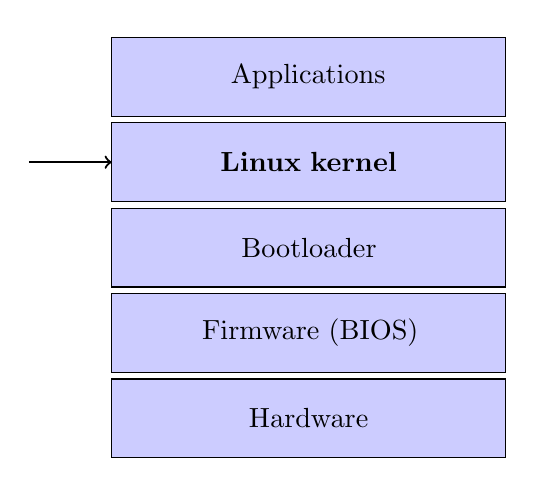
\begin{tikzpicture}
    [outer sep = 0pt, component/.style={rectangle, draw=black, fill =
      blue!20, thin, text width = 5cm, minimum height = 1cm, inner
      sep = 0pt}]
    \matrix (software_stack) [matrix of nodes, nodes in empty cells,
    column sep=2pt, row sep=2pt,
    nodes = {component, outer sep = 0pt, anchor=center, align=center}]  {
      Applications \\
      \textbf{Linux kernel} \\
      Bootloader \\
      Firmware (BIOS) \\
      Hardware \\
    };
    \draw [->, thick] ([xshift=-30pt]software_stack-2-1.west) -- (software_stack-2-1.west);
  \end{tikzpicture}  
}
\end{frame}

\begin{frame}
Building (\& installing) the kernel results in the following files being created,
\begin{itemize}
\item kernel image (\texttt{bzImage} aka \texttt{vmlinuz})
\item Initramfs image.
\item kernel modules (E.g. \texttt{ext4.ko}) \\
  Code that is pluggable at run time.
\end{itemize}
NOTE: The kernel is currently being built only for the x86 architecture.
\end{frame}

\subsection{vmlinux v/s vmlinuz}

\begin{frame}
  \begin{center}
  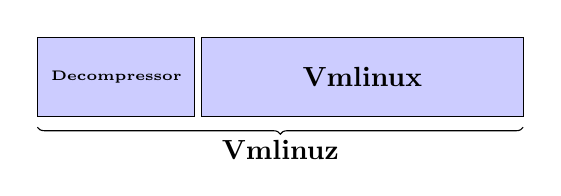
\begin{tikzpicture}
    [outer sep = 0pt, component/.style={rectangle, draw=black, fill =
      blue!20, thin, text width = 2cm, minimum height = 1cm, inner
      sep = 0pt}]

    \matrix (vmlinuz_stack) [matrix of nodes, nodes in empty cells,
    column sep=2pt, row sep=2pt,
    nodes = {component, outer sep = 0pt, anchor=center, align=center}]  {
      {\tiny \textbf{Decompressor}} \pgfmatrixnextcell \pgfmatrixnextcell \\
    };
    \node [component, fill=blue!20, fit=(vmlinuz_stack-1-2.south west)
    (vmlinuz_stack-1-3.north east), outer sep = 0pt,
    label=center:\textbf{Vmlinux}] {};

    \draw [decoration={brace, mirror}, decorate] ([yshift=-4pt]vmlinuz_stack-1-1.south
    west) -- ([yshift=-4pt]vmlinuz_stack-1-3.south east) node
    [yshift=-8pt,midway] {\textbf{Vmlinuz}};
  \end{tikzpicture}
\end{center}
  \begin{itemize}
  \item \emph{vmlinux} is the actual executable that contains the machine
    instructions that make up the kernel.
  \item \emph{vmlinuz} is generated by compressing \emph{vmlinux} and
    prefixing it with a small executable.
  \item The prefixed executable is the one which decompresses the compressed
    vmlinux image.
  \end{itemize}
\end{frame}

\subsection{Initramfs}
\begin{frame}
  \begin{itemize}
    % chandan: If we remove this, then the corresponding entry in "Further
    % reading" section should also be removed.
  \item Collection of commands and kernel modules required to mount the root
    filesystem.
  \item During boot, Linux kernel would create an in-memory filesystem and
    mount it as the root partition.
  \item The contents of the initramfs are extracted into this root partition.
  \end{itemize}
\end{frame}


\section{Set up kernel sources}
\label{sec:set-up-kernel-1}

\begin{frame}[fragile]
  \begin{itemize}
  \item Download kernel source archive
    \begin{lstlisting}
$ wget https://cdn.kernel.org/pub/linux/kernel/v4.x/linux-4.19.tar.xz
    \end{lstlisting}

  \item Extract kernel source
    \begin{lstlisting}
$ tar xvf linux-4.19.tar.xz 
$ cd linux-4.19/
    \end{lstlisting}
  \end{itemize}
\end{frame}

\section{Layout of the kernel sources}
\label{sec:layout-kernel-source}

\begin{frame}[fragile]
  \begin{tabular}{ll}
    \texttt{arch} & \texttt{kernel} \\
    \texttt{block} & \texttt{lib} \\
    \texttt{certs} & \texttt{LICENSES} \\
    \texttt{COPYING} & \texttt{MAINTAINERS} \\
    \texttt{CREDITS} & \texttt{Makefile} \\
    \texttt{crypto} & \textbf{\texttt{mm}} \\
    \textbf{\texttt{Documentation}} & \textbf{\texttt{net}} \\
    \textbf{\texttt{drivers}} & \texttt{README} \\
    \texttt{firmware} & \texttt{samples} \\
    \textbf{\texttt{fs}} & \texttt{scripts} \\
    \texttt{include} & \texttt{security} \\
    \texttt{init} & \texttt{sound} \\
    \texttt{ipc} & \texttt{tools} \\
    \texttt{Kbuild} & \texttt{usr} \\
    \texttt{Kconfig} & \texttt{virt} \\
  \end{tabular}
\end{frame}

\section{Makefile example}
\label{sec:makefiles}

\begin{frame}[fragile]
  \begin{itemize}
  \item \texttt{add.h}
\begin{lstlisting}
#ifndef _ADD_H
#define _ADD_H

int add(int n1, int n2);

#endif
\end{lstlisting}
  \item \texttt{add.c}
\begin{lstlisting}
#include "add.h"

int add(int n1, int n2)
{
        return n1 + n2;
}
\end{lstlisting}
  \end{itemize}
\end{frame}

\begin{frame}[fragile]
  \begin{itemize}
  \item \texttt{main.c}
\begin{lstlisting}
#include <stdio.h>
#include <stdlib.h>
#include "add.h"

int main(void)
{
        int sum;

        sum = add(3, 3);

        printf("sum = %d.\n", sum);

        exit(0);
}
\end{lstlisting}
  \end{itemize}
\end{frame}

\subsection{Makefile syntax}
\begin{frame}[fragile]
  \begin{itemize}
  \item A Makefile consists of a sequence of rules
  \item Each rule has the following syntax,
\begin{lstlisting}
TARGET : PRE-REQUISITES
<TAB> COMMAND1
<TAB> COMMAND2
<TAB> ...
<TAB> COMMANDN
\end{lstlisting}
  \end{itemize}
\end{frame}


\begin{frame}[fragile]
  \begin{itemize}
  \item Makefile
\begin{lstlisting}
main : main.o add.o add.h
        cc -o main main.o add.o

main.o : main.c add.h
        cc -c main.c

add.o : add.c add.h
        cc -c add.c

list_etc :
        @echo "/etc contents:"
        ls /etc
\end{lstlisting}
  \end{itemize}
\end{frame}

\section{Linux kernel Makefiles}

\begin{frame}[fragile]
  \begin{itemize}
  \item Contains sequence of commands to build the source code in
    order to generate the kernel image, kernel modules, etc.
  \item Think of Makefiles as recipes of instructions on how to build the
    kernel.
  \item Each subdirectory contains its own Makefile which invokes commands to
    build modules from source code.
\begin{lstlisting}
$ ls virt/
kvm  lib  Makefile
\end{lstlisting}
  \item The top level Makefile invokes Makefiles in each of the sub directories
    and collates some of the kernel modules to generate the kernel image.
  \end{itemize}
\end{frame}

\section{Configure kernel build}
\label{sec:configure-kbuild}

\begin{frame}[fragile]
  \begin{itemize}
  \item ... AKA How do Makefiles determine which parts of the kernel sources must be built,
    \begin{itemize}
    \item As part of the kernel image
    \item And which ones should be built as kernel modules.
    \end{itemize}
  \item A \texttt{.config} file contains the above information.
  \item Let's generate the \texttt{.config} file with default/recommended
    values.
    \begin{lstlisting}
$ make localmodconfig
LEX     scripts/kconfig/zconf.lex.c
HOSTCC  scripts/kconfig/zconf.tab.o
HOSTLD  scripts/kconfig/conf
#
# configuration written to .config
#
\end{lstlisting}
  \item Let's start building the \textbf{kernel image}.
\end{itemize}
\end{frame}

\begin{frame}[fragile]
  \begin{itemize}
\item Sample entries from the default .config file.
  \begin{itemize}
  \item \texttt{CONFIG\_X86\_PKG\_TEMP\_THERMAL=m} \\
    Indicates that \emph{Thermal driver} code should be built as a separate module.
  \item \texttt{CONFIG\_EXT4\_FS=y} \\
    Indicates that \emph{Ext4} code should be made part of bzImage.
  \item \texttt{\# CONFIG\_EXT4\_ENCRYPTION is not set} \\
    Do not build \emph{Encryption} feature of Ext4; Not even as a module.
    % HINT: Ask the audience to not focus on the details of each entry inside
    % .config.
  \end{itemize}
\begin{lstlisting}
\end{lstlisting}
\end{itemize}
\end{frame}

\begin{frame}[fragile]
    \begin{lstlisting}
$ make menuconfig
    \end{lstlisting}
  \begin{figure}[h!]
    \centering
    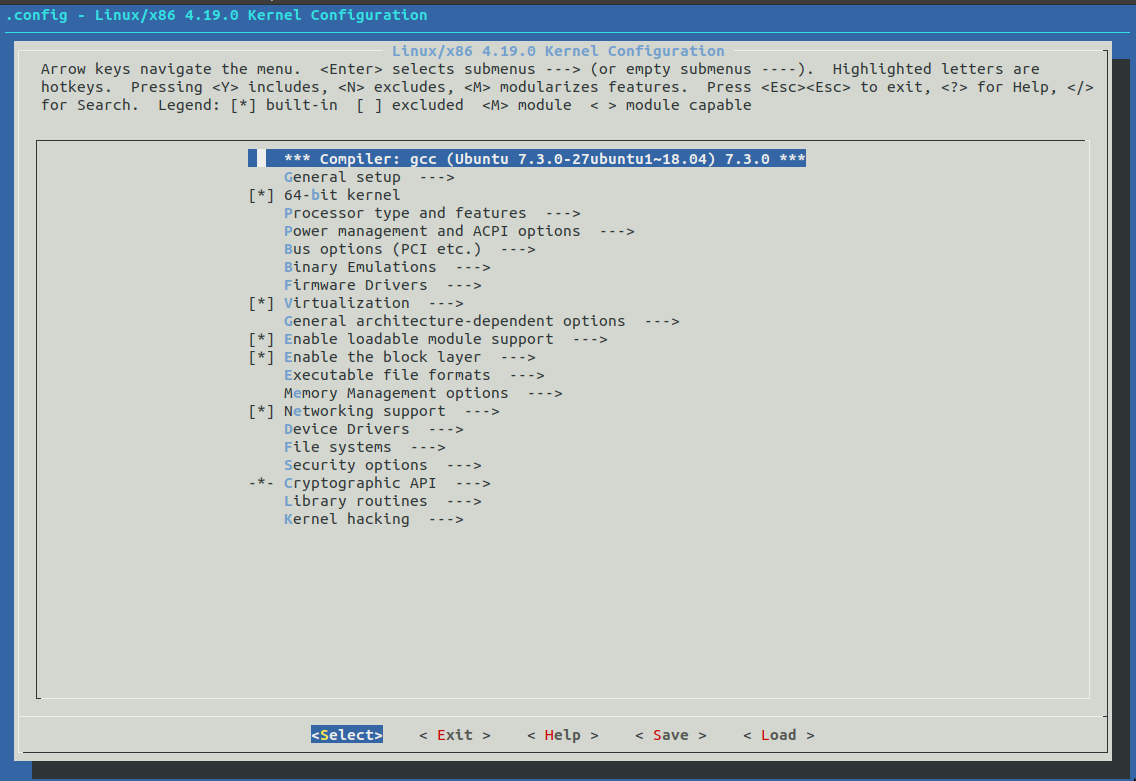
\includegraphics[scale=0.3]{images/make-menuconfig.png}
  \end{figure}
\end{frame}

\subsection{Example: Enable access to .config via /proc}
\begin{frame}
  \begin{figure}[h!]
    \centering
    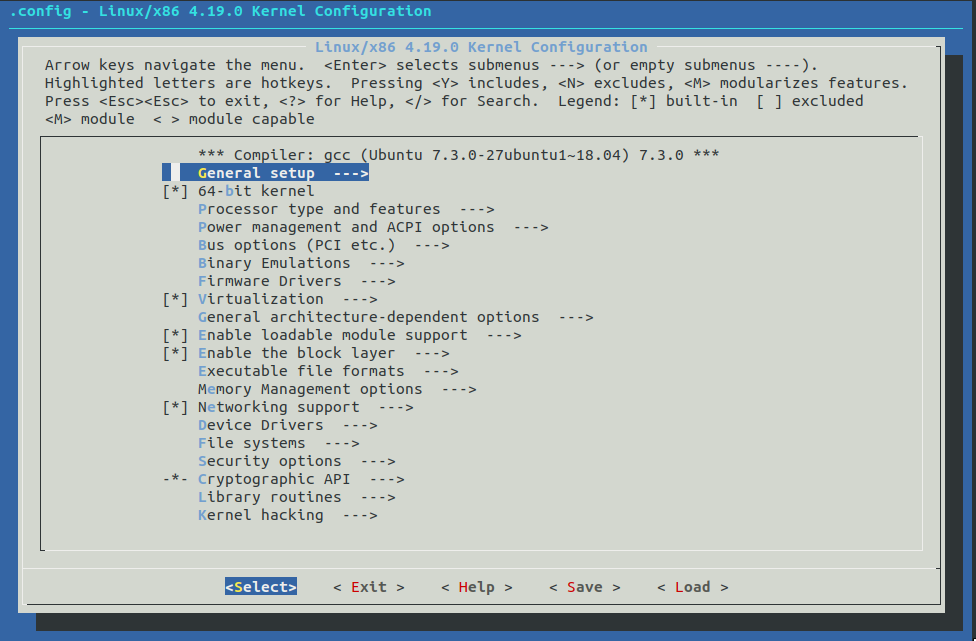
\includegraphics[scale=0.3]{images/proc-config-0.png}
  \end{figure}
\end{frame}

\begin{frame}
  Type \texttt{/} (Forward slash character) to search.
  \begin{figure}
    \centering
    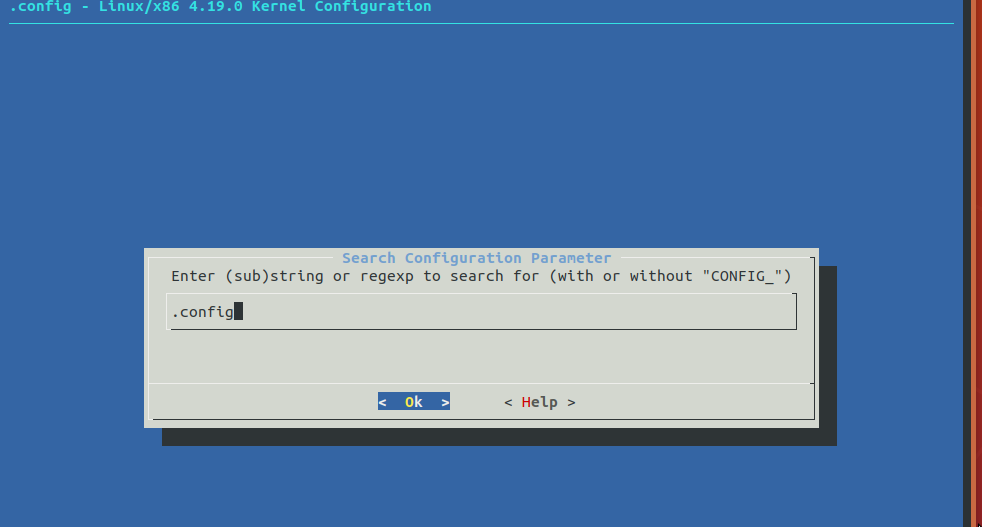
\includegraphics[scale=0.4]{images/proc-config-0-1.png}
  \end{figure}
\end{frame}

\begin{frame}
  The search results will display the path to navigate in order to get to the
  config option.
  \begin{figure}[h!]
    \centering
    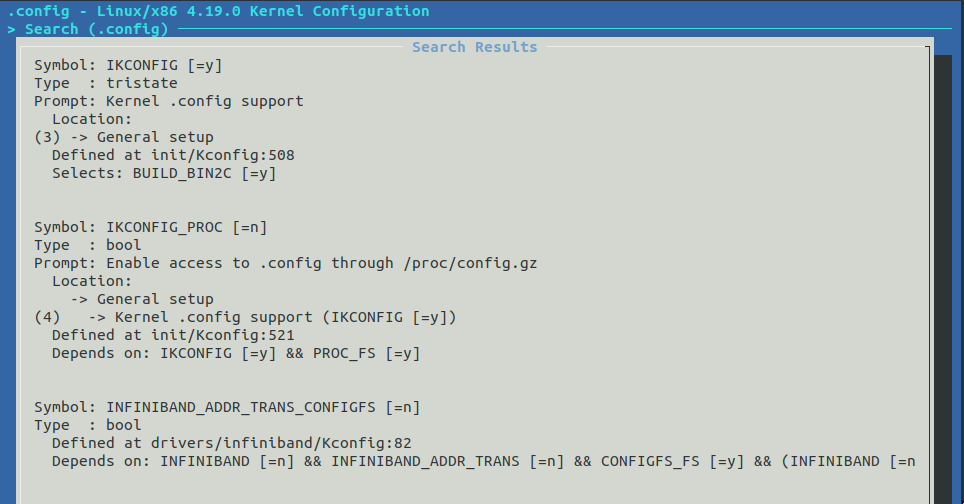
\includegraphics[scale=0.4]{images/proc-config-0-2.png}
  \end{figure}
\end{frame}

\begin{frame}
  \begin{figure}[h!]
    \centering
    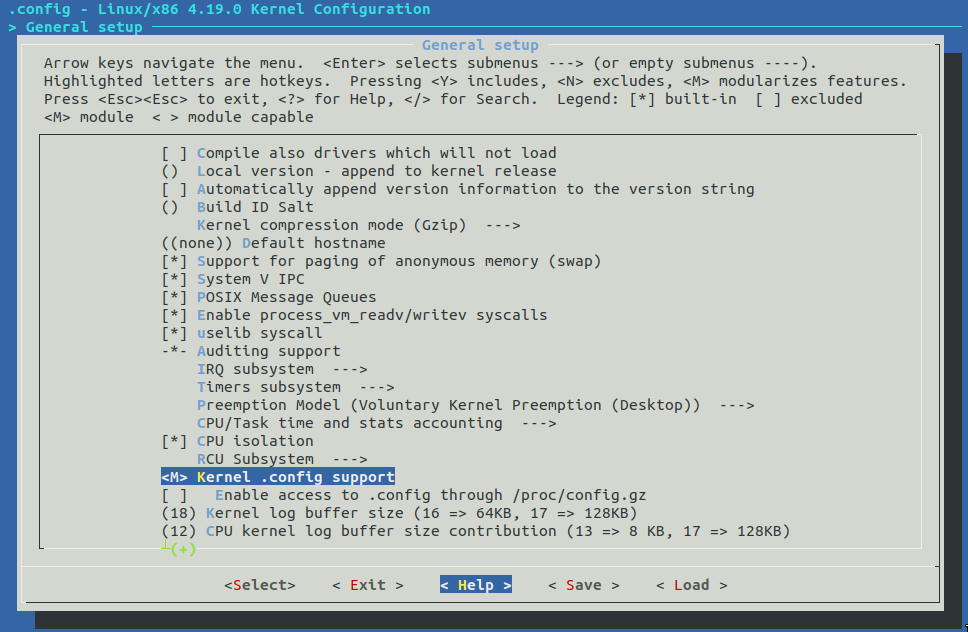
\includegraphics[scale=0.3]{images/proc-config-1.png}
  \end{figure}
\end{frame}

\begin{frame}
  \begin{figure}[h!]
    \centering
    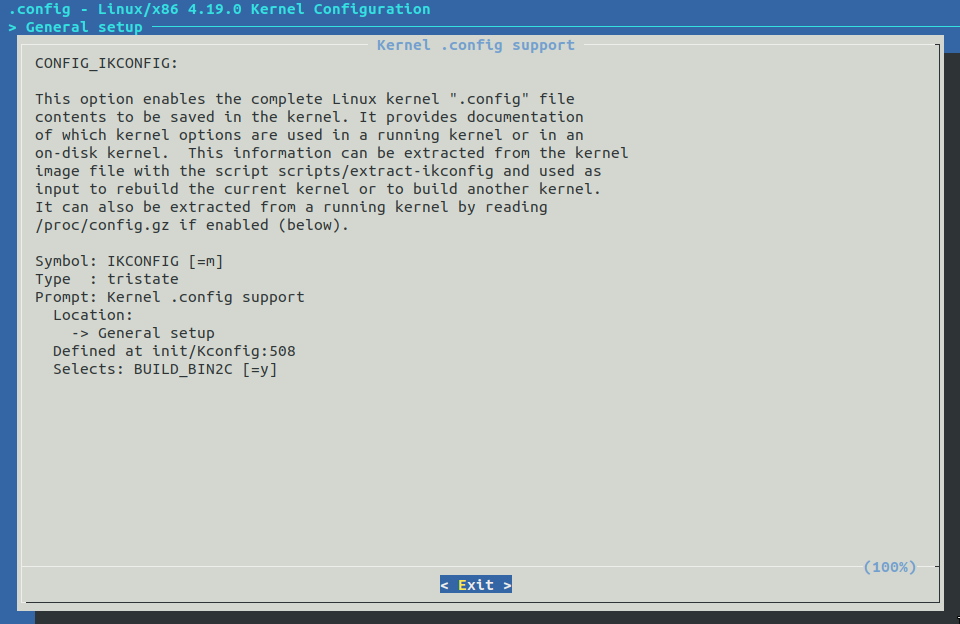
\includegraphics[scale=0.3]{images/proc-config-2.png}
  \end{figure}
\end{frame}


\begin{frame}
  \begin{figure}[h!]
    \centering
    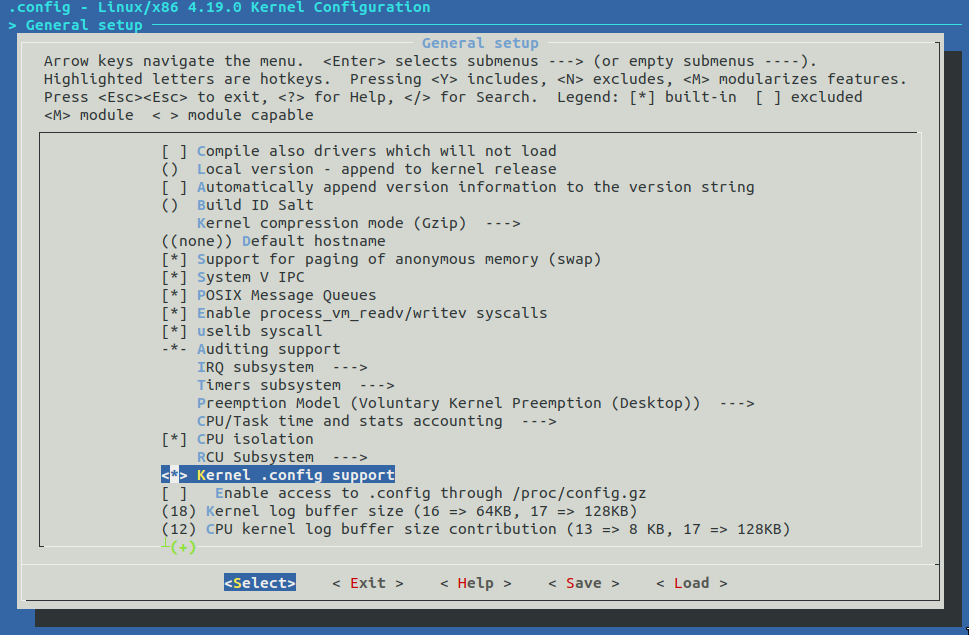
\includegraphics[scale=0.3]{images/proc-config-3.png}
  \end{figure}
\end{frame}

\section{Build and install the kernel}

\begin{frame}[fragile]
\begin{itemize}
\item Build the kernel image.
  \begin{lstlisting}
    $ make bzImage
  \end{lstlisting}

\item Build kernel modules
  \begin{lstlisting}
    $ make modules
  \end{lstlisting}
  
\item Install the kernel modules
  \begin{lstlisting}
    $ make modules_install
  \end{lstlisting}
  The kernel modules built are copied to {\tiny\texttt{/lib/modules/<kernel-version>/}}

\item Install the kernel image
  \begin{lstlisting}
    $ make install
  \end{lstlisting}
  \begin{itemize}
  \item Copies bzImage to {\tiny \texttt{/boot/vmlinuz-<kernel-version>}}.
  \item Builds the corresponding initramfs
    i.e. {\tiny \texttt{/boot/initramfs-<kernel-version>}}.
  \item Adds an entry into the bootloader's configuration file i.e. {\tiny \texttt{/boot/grub2/grub.cfg}}.
  \end{itemize}
\end{itemize}
\end{frame}

\section{Dmesg - Kernel communicates with the user}
\subsection{Introduction to printk()}
\begin{frame}
  \begin{itemize}
  \item \texttt{printk()} is a function provided to print data from the kernel
    code.
  \item Has similar semantics to Standard C library's \texttt{printf()}.

  \item \texttt{printk()} dumps its contents to a ring buffer maintained by
    the kernel.
  \item For example, Lets add a call to \texttt{printk()} inside the function
    \texttt{\_do\_fork()} (defined in \texttt{kernel/fork.c}),

  {\centering \texttt{ printk("\%s is creating another process.",
      current->comm);}} 
\item The corresponding output can be seen on the console.
  \end{itemize}
\end{frame}

\begin{frame}
  \begin{itemize}
  \item \texttt{dmesg} utility helps us extract the contents of kernel's ring
    buffer and prints the contents on the terminal.
  \item Example invocation:
    \begin{figure}[h!]
      \centering
      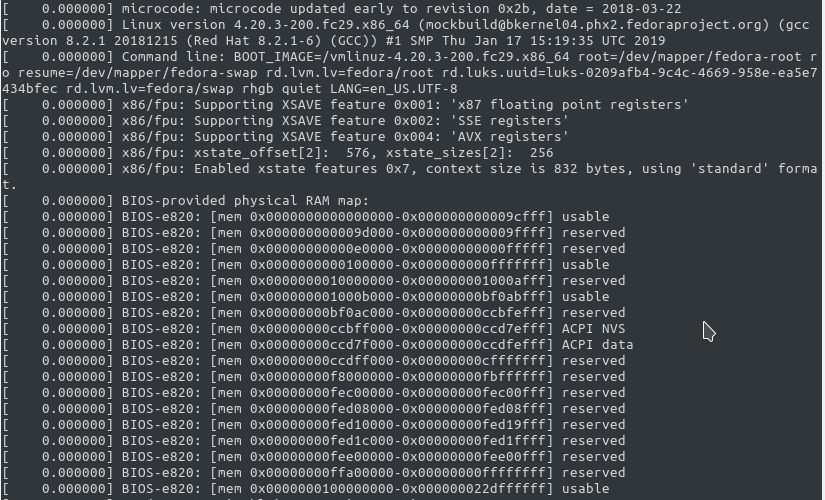
\includegraphics[scale=0.3]{images/dmesg-0.png}
    \end{figure}
  \end{itemize}
\end{frame}

\section{Assignment}
\begin{frame}[fragile]
  \begin{itemize}
  \item \texttt{uname} extracts information about the currently running
    kernel.
  \item Example interaction,
\begin{lstlisting}
$ uname -s # Kernel name
Linux
$ uname -r # kernel release
4.20.3-200.fc29.x86_64
$ uname -v # kernel version
#1 SMP Thu Jan 17 15:19:35 UTC 2019
$ uname -m # Architecture
x86_64
\end{lstlisting}
  \end{itemize}
\end{frame}

\begin{frame}
  Configure, build and boot the Linux kernel such that the output of the
  command \texttt{uname -r} has your name suffixed to the original value. 
    \begin{figure}[h!]
      \centering
      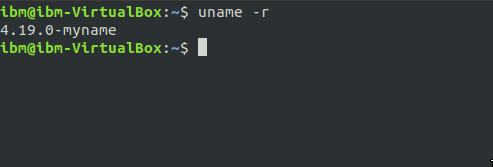
\includegraphics[scale=0.5]{images/assignment.png}
    \end{figure}
    HINT: Search for the string \texttt{version} in the interface provided by
    \texttt{make menuconfig}.
\end{frame}

\section{Further reading}
\begin{frame}
  \begin{itemize}
  \item Kernel build configuration:
    { \tiny https://www.youtube.com/watch?v=M-Nx3-p6T7k }
  \item Initramfs: {\tiny  http://www.linuxfromscratch.org/blfs/view/svn/postlfs/initramfs.html}
  \item Makefile: { \tiny https://en.wikipedia.org/wiki/Makefile }
  \end{itemize}
\end{frame}

\end{document}

%%% Local Variables:
%%% mode: latex
%%% TeX-master: t
%%% End:
